\documentclass[12pt,spanish,a4paper]{book}
\usepackage{geometry}
\geometry{
	a4paper,
	total={170mm,257mm},
	left=20mm,
	top=20mm,
}
\usepackage[utf8]{inputenc}
\usepackage{babel}
\usepackage{graphicx}
\graphicspath{ {imagenes/} }
\usepackage{amsmath}
\usepackage{graphicx}
\usepackage{wrapfig}
\usepackage{parskip}
\usepackage{listings}
\usepackage[obeyspaces]{url}
\usepackage{caption}
\usepackage{subcaption}
\addto\captionsspanish{
    \def\listtablename{\'Indice de tablas}%
    \def\tablename{Tabla}
}
\usepackage{multirow}
\usepackage{textcomp} % ° symbol
\usepackage{amsmath}
\usepackage{float}
\usepackage[breaklinks=true,hidelinks]{hyperref} 

% \say para las comillas
\usepackage{dirtytalk}

% cases
\usepackage{mathtools}

% debug packages
\usepackage{xcolor}
\usepackage{afterpage}
\newcommand\blankpage{%
    \null
    \thispagestyle{empty}%
    \addtocounter{page}{-1}%
    \newpage}

% Palatino font type
\usepackage[T1]{fontenc}
\usepackage{mathpazo}

% Interlineado
\usepackage{setspace}
\onehalfspacing

% Sangría
\setlength\parindent{12pt}

% colores nord blues
\definecolor{mycolor}{RGB}{94, 129, 172} % nord blue
\definecolor{mylcolor}{RGB}{129, 161, 193} % nord lighter blue

% color de las secciones
\usepackage{sectsty}
\chapterfont{\color{mycolor}}
\sectionfont{\color{mycolor}}
\subsectionfont{\color{mycolor}}
\subsubsectionfont{\color{mycolor}}
\let\oldtextbf\textbf
\renewcommand{\textbf}[1]{\textcolor{mycolor}{\oldtextbf{#1}}}

% línea horizontal debajo de las secciones
\usepackage{titlesec}
\titleformat{\section}
  {\normalfont\Large\bfseries\color{mycolor}}
  {\thesection}{1em}{}[{\titlerule[0.8pt]}]

% index
\usepackage{imakeidx}
\makeindex[columns=3, title=Alphabetical Index, intoc]


\begin{document}

\frontmatter % enumeración de las páginas con números romanos

\blankpage
\blankpage

% Carátula
\thispagestyle{empty}
\begin{center}
{\large

    \vspace{1cm}

    {\Huge Simulaciones computacionales para el desarrollo de electrodos de 
            baterias de ion-litio de próxima generación}
    
    \vspace{0.5cm}
    por
    \vspace{0.5cm}
    
    {\Large Francisco Fernandez}

    \vspace{0.5cm}

    Presentado ante la Facultad de Matemáticas, Astronomía, Física y Computación 
    como parte de los requerimientos para la obtención del grado de
    
    \vspace{0.5cm}

    {\Large Doctor en Física}

    \vspace{0.5cm}
    de la

    UNIVERSIDAD NACIONAL DE CÓRDOBA

    \vspace{0.5cm}
    % logo 
    
    mes, 202?

    \textcopyright FaMAF - UNC 202?

    \vspace{1.5cm}

    Director: Daniel Eugenio Barraco Díaz

    Codirector: Ezequiel Pedro Marcos Leiva

    % licencia
}
\end{center}

% Dedicatoria

% Índice
\tableofcontents

% Resumen

% Abstract

% Capítulos...

\mainmatter % a partir de acá se cuentan los números de las páginas en formato arabico

% \chapter[Capítulo X]{Capítulo X}
% \input{corpus/capitulox.tex}
\chapter[Teoría y métodos computacionales]{Teoría y métodos computacionales}
\section{Breve introducción a la mecánica estadística}

En la mayoría de los experimentos que se realizan en un laboratorio se obtiene 
una serie de mediciones sobre sistemas macroscópicos, usualmente constituidos por 
más de 10$^{20}$ moléculas, durante un período de tiempo, a las cuales luego se 
les realiza un promedio. La mecánica estadística ofrece una interpretación de 
las propiedades del equilibrio de sistemas macroscópicos a partir de una teoría 
molecular aplicada a su configuración microscópica ~\cite{hill1986}.

Si se quisiera calcular alguna variable mecánica de un sistema termodinámico a
partir de consideraciones moleculares tendríamos que hacerlo durante un período
de tiempo largo para suavizar las fluctuaciones y para que fuera independiente
del paso inicial a la hora de realizar el promedio. Dado el gran número de 
moléculas interactuantes entre sí en estos sistemas, este cálculo está fuera de
alcance tanto en una consideración cuántica como en una clásica. Una alternativa
para solucionar esto es conectar el promedio temporal de la variable mecánica de
interés con el promedio de ensambles, donde un ensamble es simplemente una 
colección de un número muy largo de sistemas construidos de manera tal que 
reproducen las propiedades termodinámicas del sistema en cuestión. Si bien todos
los sistemas en el ensamble son idénticos desde el punto de vista termodinámico,
no lo son en sus configuraciones moleculares. De esta manera ahora se tiene
que el valor promedio de la variable mecánica en estudio se realiza sobre estas 
replicas del sistema en vez de sobre su evolución temporal.

\subsection{Ensambles}

Algunos de los ensambles termodinámicos más relevantes son:
\begin{enumerate}
    \item \textit{Ensamble microcanónico (NVE)}, un sistema aislado en el cual el 
        número de partículas, el volumen y la energía permanecen constantes.
    \item \textit{Ensamble canónico (NVT)}, un sistema cerrado, con una cantidad
        fija de partículas y volumen constante, en contacto con un baño de 
        temperatura lo suficientemente grande de manera tal que la misma permanece 
        constante.
    \item \textit{Ensamble gran canónico ($\mu$VT)}, un sistema abierto en el que
        el volumen está fijo, se está en contacto con un baño de temperatura y
        además se permite el intercambio de partículas con un reservorio.
    \item \textit{Ensamble isotérmico-isobárico (NPT)}, en este sistema el número
        de partículas está fijo y en contacto con un baño de temperatura y un
        pistón que permite variar el volumen para mantener la presión constante.
\end{enumerate}

\subsection{Hipótesis ergódica}

El primer postulado de la Mecánica estadística presentado en esta tesis es 
referido como la \textbf{hipótesis ergódica} y nos dice que \textit{El promedio 
temporal de una variable mecánica $M$ en el sistema termodinámico de interés es 
igual al promedio de ensambles de M, en el límite del conjunto de ensambles que 
tiende a infinito, siempre que los sistemas del conjunto de ensambles reproduzcan 
el estado termodinámico y el entorno del sistema real de interés}. Es decir que
es lo mismo calcular el promedio en la evolución temporal que en una cantidad 
grande estructuras instantáneas representativas del sistema. Para poder aplicar
este postulado se necesita conocer la probabilidad relativa de cada uno de los 
estados presentes en el ensamble.

\subsection{Postulado de igual probabilidad a priori}

El segundo postulado de la Mecánica estadística presentado se refiere a esto
último y establece que \textit{En un conjunto de ensambles representativo de un 
sistema termodinámico aislado, los sistemas del conjunto de ensambles se distribuyen 
uniformemente, es decir, con igual probabilidad o frecuencia, sobre los posibles 
estados con los valores especificados de dicho sistema termodinámico aislado}.
En otras palabras, cada estado esta representado por la misma cantidad de sistemas
en el ensamble.

\subsection{Fluctuaciones}

Para definir el valor medio (o examinar la amplitud de las fluctuaciones en torno 
al valor medio) de una propiedad de un sistema que puede existir en varios estados
$j$ con probabilidades $P_j$, la propiedad misma debe definirse en cada estado 
$j$. Una propiedad que cumpla estos criterios es \say{mecánica} por definición.

Tomemos el ejemplo de la fluctuación de la energía de un sistema cerrado en 
contacto con un reservorio de temperatura lo suficientemente grande (NVT) donde 
las fluctuaciones de energía deben estar asociadas al intercambio de calor entre 
el sistema y el reservorio. Estas fluctuaciones de energía resultan ser muy 
pequeñas, por lo que la función de distribución de probabilidad para las 
diferentes energías tiene forma gaussiana en torno al valor medio $\overline{E}$. 
La dispersión en esta distribución de probabilidad puede, por lo tanto,
caracterizarse completamente por la desviación estándar $\sigma_E$, es decir, 
$$
\sigma_E = \sqrt{\overline{(E - \overline{E})^2}}.
$$

Si diferenciamos
$$
\overline{E} \sum_j e^{-E_j(N,V)/kT} = \sum_j E_j(N,V) e^{-E_j(N,V)/kT}
$$
con respecto a $T$, y luego dividimos por $Q$, la función de partición, encontramos
$$
\left(\frac{\partial\overline{E}}{\partial T}\right)_{V,N} + \frac{\overline{E}}{Q kT^2} \sum_j E_j e^{-E_j / kT} = \frac{1}{Q kT^2} \sum_j E_j^2 e^{-E_j/kT},
$$
o
$$
\overline{E^2} - (\overline{E})^2 = \overline{(E-\overline{E})^2} = \sigma_E^2 = k T^2 C_V,
$$
de la termodinámica, sabemos que en general $C_V \approx \mathcal{O}(Nk)$ and $\overline{E} \approx \mathcal{O}(NkT)$. Por lo tanto
\begin{equation}\label{eq:fluctuaciones}
    \frac{\sigma_E}{\overline{E}} = \frac{\sqrt{kT^2C_V}}{\overline{E}} \approx \mathcal{O}(N^{-1/2})
\end{equation}
Así encontramos en un sistema típico cerrado e isotérmico el comportamiento de la
desviación estándar de la distribución de probabilidad de la energía.

Las variables que fluctúan son diferentes en cada ensamble, aunque las funciones 
termodinámicas calculadas en mecánica estadística resultan ser independientes del 
ensamble utilizado en el cálculo, por lo cual, pueden realizarse análisis 
similares en las distintas cantidades que pueden variar en cada uno de ellos.

En el límite termodinámico, en el cual la cantidad de moléculas en un sistema es 
del orden de $10^{23}$, la relación obtenida en la ecuación \ref{eq:fluctuaciones} 
muestra que las fluctuaciones son muy pequeñas y pueden ser ignoradas. Esto hace 
que los ensambles sean termodinámicamente equivalentes entre sí.

En termodinámica, las relaciones funcionales entre las variables termodinámicas 
de un sistema son independientes del entorno. Otra forma de decir esto es que la 
elección de las variables termodinámicas independientes es arbitraria y no está 
prescrita por el entorno. En la mecánica estadística llegamos a la misma 
conclusión: independientemente del entorno, podemos seleccionar cualquier ensambles
o función de partición que deseemos para calcular las propiedades termodinámicas; 
los resultados deben ser independientes de la elección.


\section{Dinámica molecular}\label{md}

La dinámica molecular (MD, de sus siglas en inglés, \textit{molecular dynamics})
es una técnica de simulación computacional que considera un sistema de $N$
partículas atómicas, que interactúan a través de un campo de fuerzas newtoniano,
de las cuales se obtiene su evolución temporal. La misma permite obtener
propiedades termodinámicas macroscópicas de un sistema en equilibro a partir de 
cantidades microscópicas ~\cite{frenkel2001, allen2017}.

Para entender mejor como trabaja esta técnica de simulación es conveniente ver
cómo funciona su código fuente, un diagrama de flujo del mismo es presentado en 
la figura \ref{fig:esquema_md}, donde cada una de sus partes se amplía en la 
siguiente enumeración:
\begin{enumerate}
    \item \textbf{Inicialización del sistema}: se especifican las posiciones y
        velocidades iniciales de los átomos. También se elije un paso temporal, 
        un radio de corte para las interacciones y las condiciones de contorno que
        se van a respetar a lo largo de la simulación. 
    \item \textbf{Cálculo de fuerzas}: con las posiciones especificadas se
        calcula la fuerza sobre cada uno de los átomos a través del campo de 
        fuerzas elegido.
    \item \textbf{Integración de las ecuaciones de movimiento}: se integran las
        ecuaciones de Newton mediante algún integrador que obtiene las posiciones
        y velocidades del paso temporal siguiente a partir del actual.
    \item \textbf{Cómputo de propiedades termodinámicas}: se realizan los
        cálculos de distintas cantidades de interés, como las energías potencial
        y cinética, la presión y la temperatura.
    \item De ser necesario, se aplica algún \textbf{termostato o barostato}
        para realizar simulaciones en el ensamble termodinámico deseado.
    \item \textbf{Evolución temporal}: se incrementa el tiempo adhiriendo un
        paso temporal y se vuelve al cálculo de las fuerzas con las nuevas 
        configuraciones.
\end{enumerate}

\begin{figure}
    \centering
    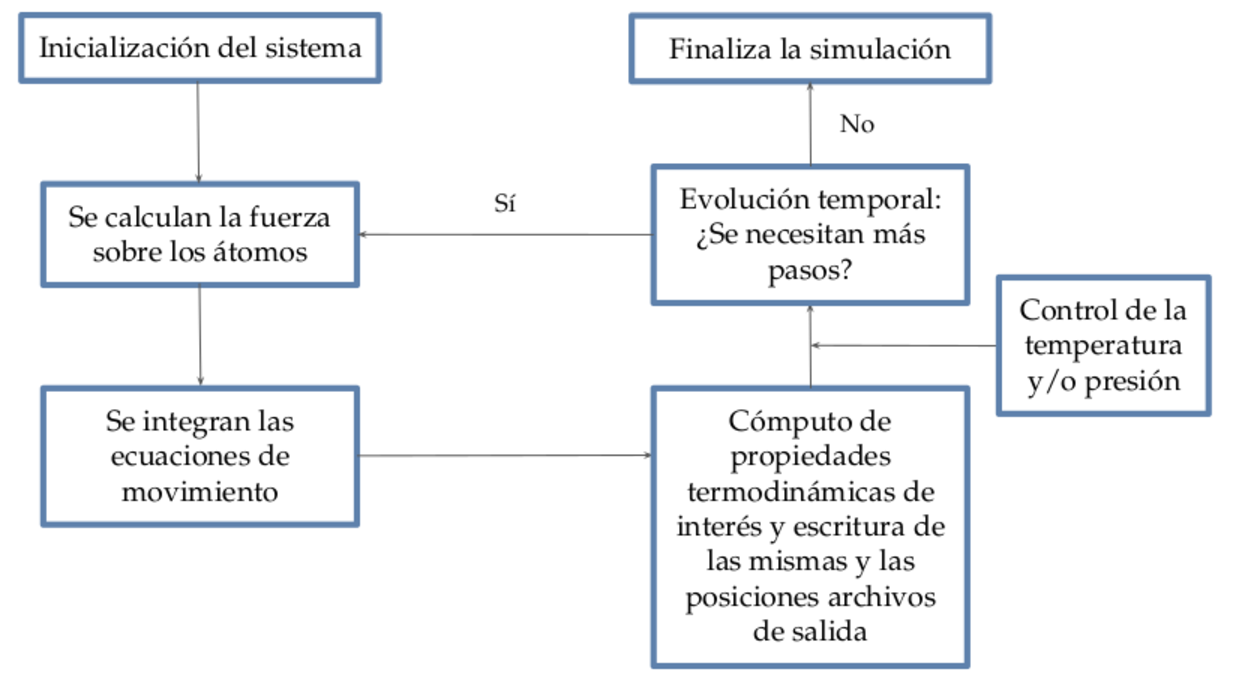
\includegraphics[width=\textwidth]{metodos/esquema_de_dinamica_molecular.pdf}
    \caption{Esquema de un diagrama de flujo de una dinámica molecular usual.}
    \label{fig:esquema_md}
\end{figure}

A continuación se especifican cada una de dichas partes con mayor detenimiento.

\subsection{Configuraciones iniciales}

Si bien las posiciones iniciales de algunos sistemas pueden reproducirse a partir
de los vectores de red de estructuras cristalinas (\textit{simple cubic}, 
\textit{body-centered cubic}, \textit{face-centered cubic}), otros casos de
interés, en los cuales hay más de un elemento involucrado, involucran celdas 
unidad más complicadas que han sido calculadas y optimizadas mediante la Teoría
del funcional de la densidad electrónica (DFT, de sus siglas en inglés, density 
functional theory). Realizar estos cálculos suele ser una tarea computacionalmente 
costosa y que requiere intervención de científicos especializados, para evitar esto
existe una base de datos ampliamente utilizada en el ámbito académico y en
la industria, Materials Project \cite{materials_project}, que recopila los datos
que existen sobre estas estructuras cristalinas, realiza nuevos cálculos y está 
abierta a la comunidad para su uso y colaboración. Antes de que los datos se
carguen en la página, los mismos son comparados con resultados experimentales 
para determinar si están dentro de un rango de validez definido. En esta tesis
en particular, fueron utilizadas distintas estructuras cristalinas de esta base de
datos como condiciones iniciales para las posiciones y el tamaño de la celda de 
simulación.

Las velocidades de los átomos suelen ser generadas de manera aleatoria, a través
de un generador de números pseudo-aleatorio, tomando como argumento una semilla 
para la reproducibilidad de la simulación y una temperatura deseada para el
sistema. Estos números suelen ser generados de una distribución gaussiana, donde
el centro se lo fija a cero para que no haya una velocidad en el centro de masa
y el ancho está relacionado a la temperatura.

\subsection{Condiciones de contorno}

Además de dar la configuración inicial de los átomos, es necesario especificar si
los mismos se encuentran dentro de una celda de simulación con un largo tamaño en
particular para cada una de las direcciones del sistema o si no interactúan fuera
del borde de la estructura que conforman los mismos. En el primero de los casos
se tienen condiciones periódicas de contorno (PBC, \textit{periodic boundary 
conditions}), lo que se busca con ellas es reproducir un sistema infinito, para
que no existan efectos de borde, y consiste en considerar que los átomos se 
encuentran dentro de una celda unidad de una red infinita de celdas idénticas; en
donde si un átomo sale por un extremo de la celda, ingresa por el opuesto. Una
condición que debe cumplir esta celda es que su tamaño en cada una de las 
direcciones debe ser mayor al radio de corte de las interacciones entre los átomos. 
Por otro lado, el segundo de los casos es útil considerarlo cuando se 
tienen nanoestructuras en las cuales los átomos están ordenados de cierta forma 
que globalmente representan una forma definida y no pueden ser consideradas como
una red infinita.

\subsection{Potenciales interatómicos}

Los potenciales interatómicos empíricos o semi-empíricos que se utilizan en las
dinámicas moleculares relacionan la fuerza sobre un átomo con el entorno químico 
del mismo a través de una forma funcional conocida. Existe una gran 
variedad de estos potenciales y la elección de uno de ellos depende del sistema 
de estudio, ya que algunos potenciales representan de mejor manera gases y otros 
metales, por ejemplo. Algunos de los potenciales interatómicos más utilizados
son mencionados brevemente a continuación. El potencial de Coulomb ~\cite{coulomb}
considera las partículas como cargas puntuales que interactúan electrostáticamente. 
El potencial de Tersoff ~\cite{tersoff} o el de Stillinger-Weber 
~\cite{stillinger-weber} fueron especialmente desarrollados para el modelado de 
materiales con enlaces covalentes fuertes, como es el caso del carbono o del 
silicio. El método del átomo embebido (EAM, de sus siglas en inglés) ~\cite{eam} 
y el EAM modificado (MEAM) ~\cite{meam} están diseñados para simular sistemas 
metálicos. Otros potenciales, como el COMB (\textit{charge-optimized many-body}) 
~\cite{comb}, que incorporan una equilibración de las cargas en el modelo, o el 
ReaxFF (\textit{reactive force fields}) ~\cite{reaxff}, que combina en un solo 
modelo distintas componentes de las que fueron mencionadas, con enfoques más 
avanzados permiten simular reacciones químicas en algunos sistemas.

Sólo a fines explicativos consideremos un potencial interatómico de Lennard-Jones
~\cite{lennard-jones}, que reproduce el decaimiento de $r^{-6}$ a distancias 
largas
dado por la siguiente expresión
$$
V_{LJ} = 4\varepsilon \left[ \left( \frac{\sigma}{r} \right)^{12} - \left( \frac{\sigma}{r} \right)^{6} \right],
$$
donde $r$ es la distancia entre dos átomos, $\varepsilon$ indica la profundidad 
del pozo del potencial que se encuentra en $r_m = 2^{1/6} \sigma$, $\sigma$ es el
radio del átomo. En la figura \ref{fig:lj} 
\begin{figure}
    \centering
    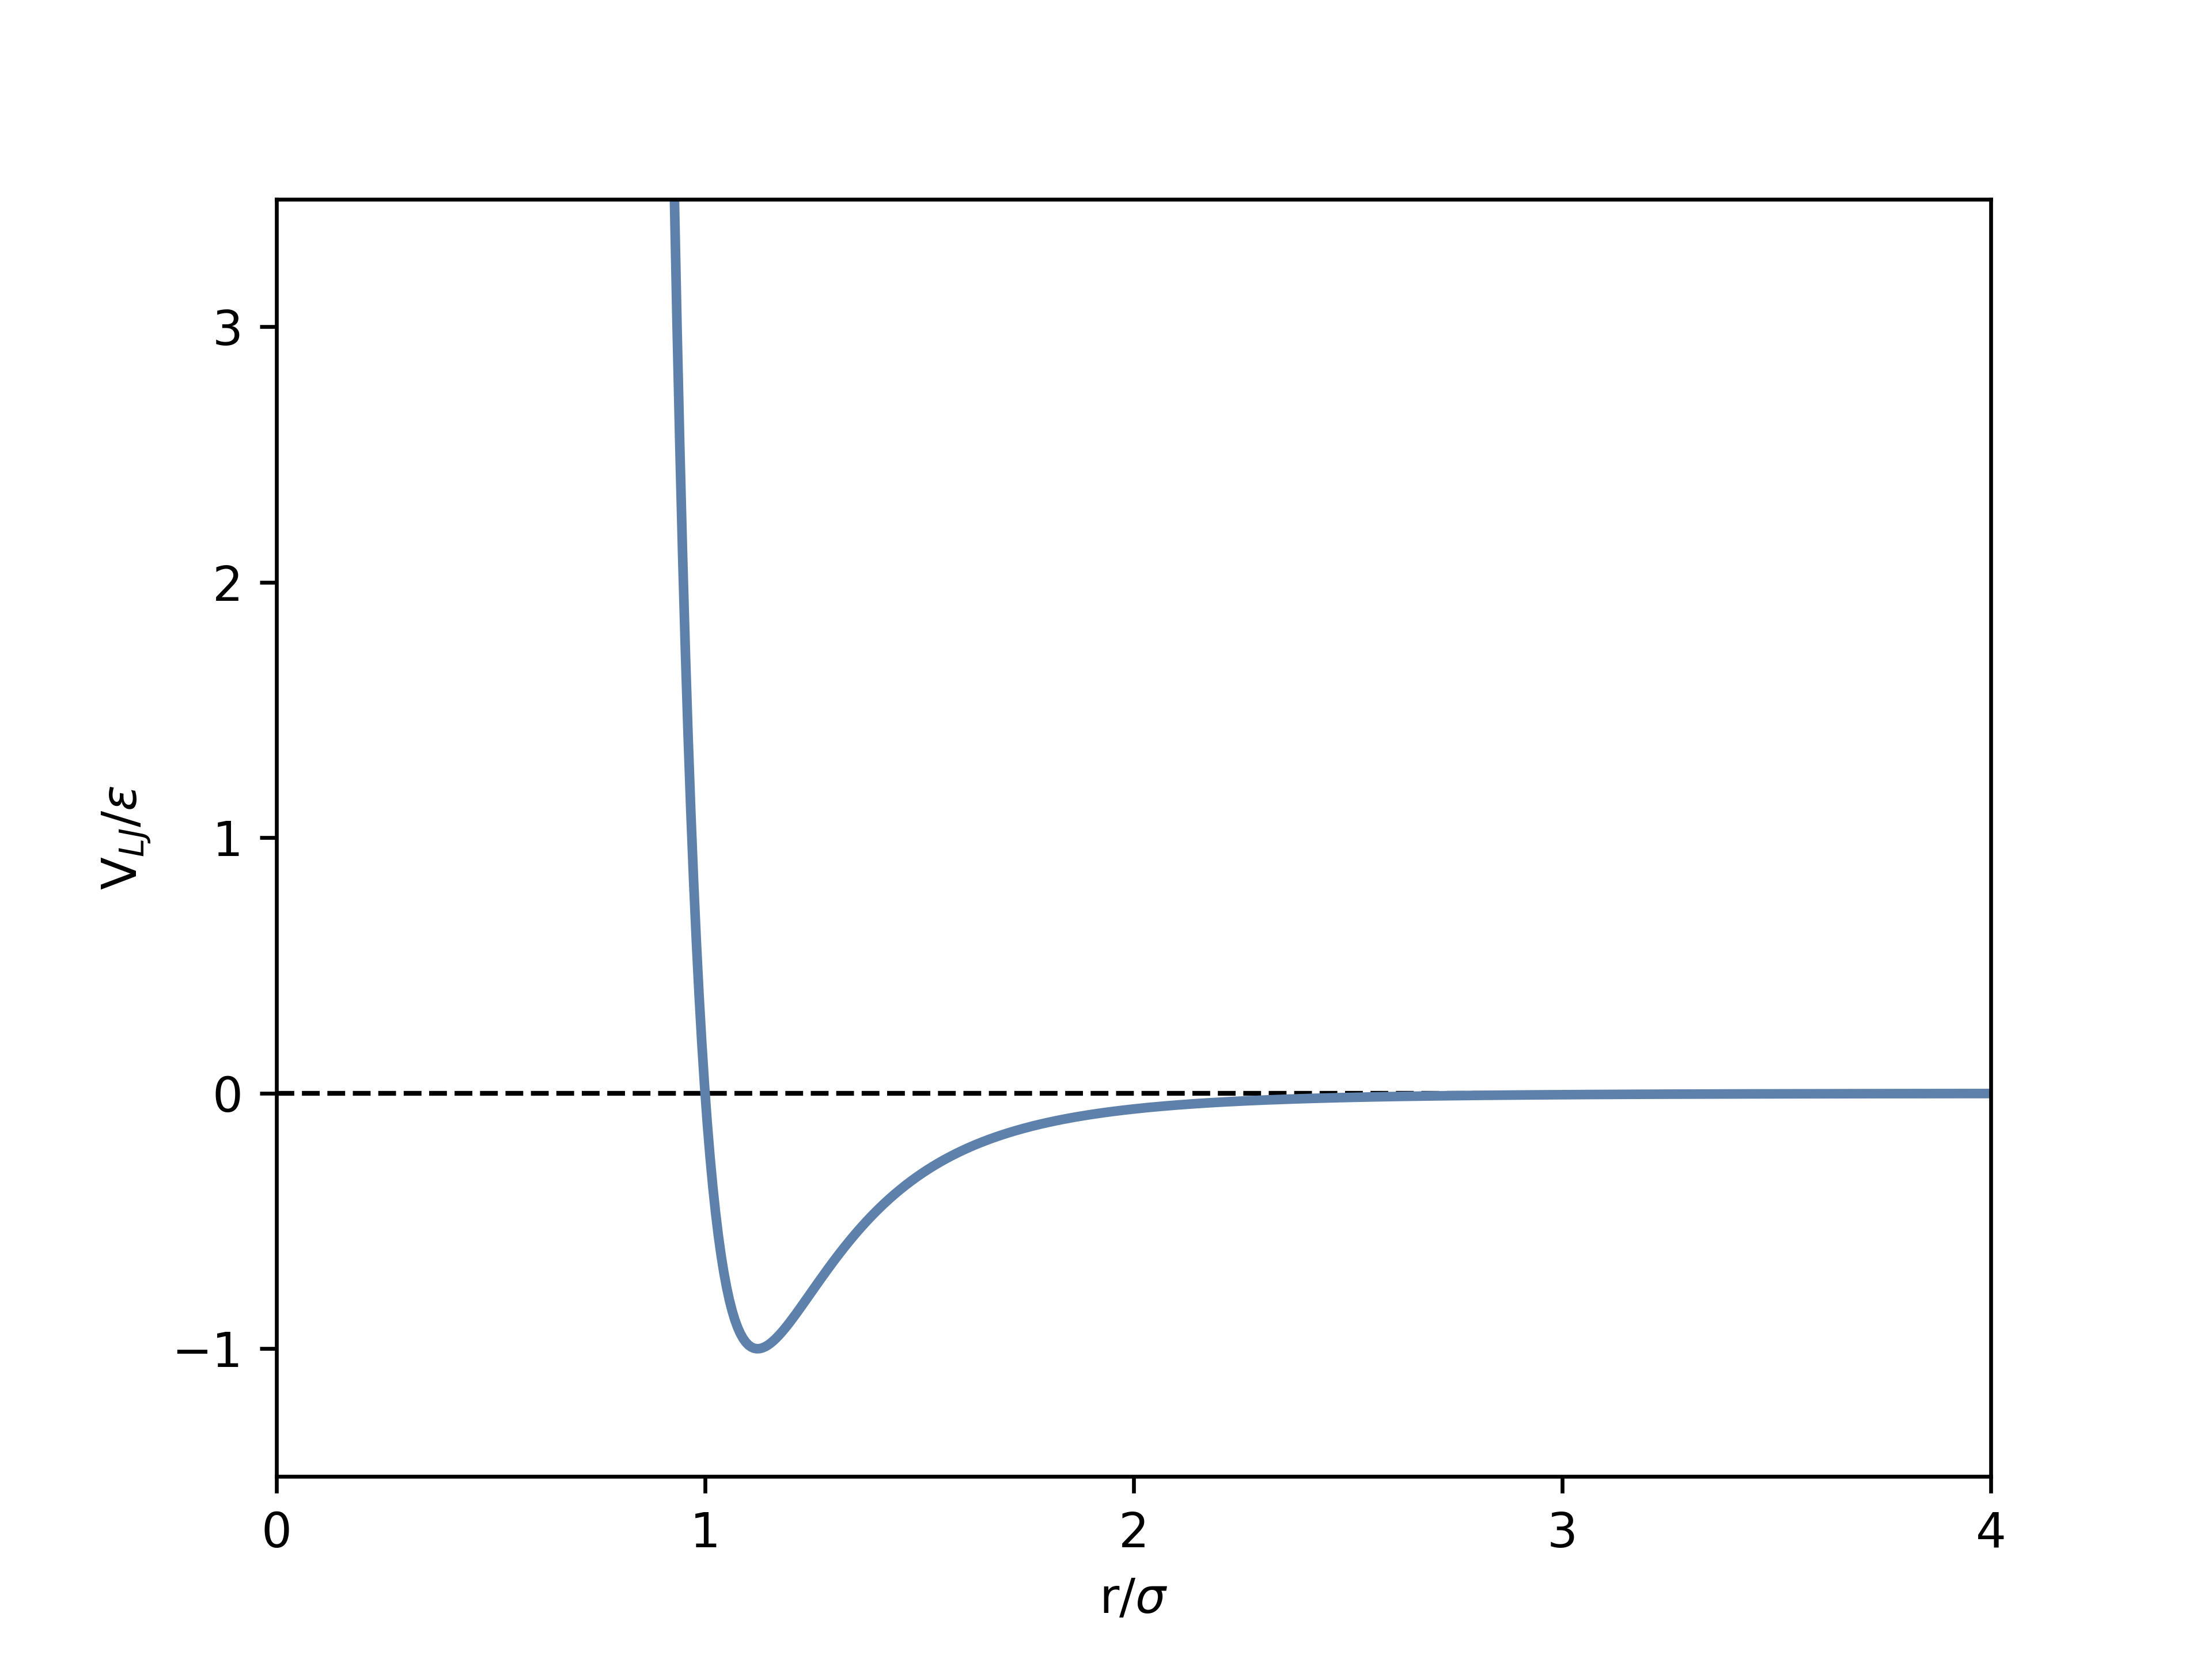
\includegraphics[width=0.7\textwidth]{metodos/lj.png}
    \caption{Gráfico de un potencial de Lennard-Jones.}
    \label{fig:lj}
\end{figure}
se muestra el comportamiento de este potencial, si la distancia entre dos
átomos es menor a $r_m$ entonces se repelen, si es mayor a dicha distancia, se 
atraen. Cuando la distancia entre dos átomos es infinita, los mismos no 
interactúan, en el caso práctico se define una distancia de corte, conocida como
el \textit{radio de corte}, $r_{cut}$, a partir de la cual se considera que el 
potencial es nulo. Para evitar discontinuidades en este punto se suelen utilizar 
distintas técnicas como el truncado y desplazado o se multiplica al potencial 
al rededor de dicho punto por una función \textit{smooth}, que hace que el 
potencial se iguale suavemente a cero.

Una vez que el potencial interatómico está bien definido, para calcular la fuerza
que actúa sobre el átomo $i$ es necesario computar la fuerza de a pares con todos
los átomos $j$ del sistema. Para esto es necesario calcular las distancias,
considerando la imagen mínima si las condiciones de contorno son PBC, y ver si
las mismas son mayores o menores a $r_{cut}$, si la distancia es mayor entonces
la contribución de esa interacción es igual a cero y si es menor se computa la 
fuerza a través del potencial de la siguiente manera
$$
f_x(r) = - \frac{\partial V(r)}{\partial x}
       = - \left( \frac{x}{r_{ij}} \right) \cdot \left( \frac{\partial V(r)}{\partial r} \right)
$$
donde $r$ es la distancia entre los átomos, $x$ la componente en alguna de
las direcciones definidas para el sistema.

A continuación se presentan dos potenciales interatómicos del estado del arte que
fueron utilizados a lo largo de esta tesis.

\subsubsection{ReaxFF}

El campo de fuerza reactivo, ReaxFF ~\cite{reaxff}, representa adecuadamente la
asociación y disociación de enlaces de átomos al considerar la energía del sistema
($E_{system}$) de manera tal que se encuentra dividida en varias contribuciones 
de energía parciales,
$$
E_{system} = E_{bond} + E_{over} + E_{under} + E_{val} + E_{pen} + E_{tors} + E_{conj} + E_{vdWaals} + E_{Coulomb}.
$$

Una de las suposiciones fundamentales del ReaxFF es que el orden de enlace entre
un par de átomos puede obtenerse directamente de la distancia que los separa, 
esto es asegurado por el término $E_{bond}$.

$E_{over}$ y $E_{under}$ son términos agregados para agregar penalidades a los
átomos sobre-coordinados o sub-coordinados, utilizando la teoría de la valencia del
enlace.

$E_{val}$ considera la contribución a la energía por el ángulo de valencia, 
mientras que $E_{pen}$ penaliza sistemas para reproducir la estabilidad de 
sistemas con dos dobles enlaces que comparten un átomo en un ángulo de valencia.

Las contribuciones a la energía de los ángulos de torsión y de los efectos de 
conjugación están dados por $E_{tors}$ y $E_{conj}$, respectivamente.

Por último, las interacciones repulsivas a distancias interatómicas cortas y 
las atractivas a distancias largas son incluidas para todos los pares de átomos
mediante un término de van der Waals, $E_{vdWaals}$, utilizando un potencial de 
Morse, y uno de Coulomb, donde las cargas de los átomos se aproximan a través de 
un método de equilibración.

Los parámetros ajustables de los potenciales ReaxFF se obtienen a partir de 
cálculos de química cuántica sobre la disociación de enlaces, reacciones de 
moléculas pequeñas, calores de formación y geometrías de distintos compuestos.

\subsubsection{DFTB}

Un método alternativo para obtener las fuerzas en dinámica molecular es a través
de la utilización de un modelo \say{híbrido} entre los métodos \textit{ab-initio},
basados en DFT, y el uso de potenciales completamente empíricos, DFTB (de sus 
siglas en inglés, \textit{Density Functional based Tight Binding}), que tiene
la ventaja de ser más transferibles que estos últimos y requiere menos costo
computacional que los primeros.

El método de DFTB se basa en una expansión de segundo orden de la energía total 
de Kohn-Sham ~\cite{dft1, dft2} en la DFT con respecto a las fluctuaciones de la 
densidad de carga. El enfoque de orden cero es equivalente a un esquema estándar 
no auto-consistente (TB), mientras que en el segundo orden se puede derivar una 
expresión transparente, libre de parámetros y fácilmente calculable para los 
elementos matriciales hamiltonianos generalizados. Estos se modifican mediante 
una redistribución auto-consistente de las cargas de Mulliken (SCC).

La energía total de un sistema de $M$ electrones en el campo de $N$ núcleos en
las posiciones $\mathbf{R}$ puede escribirse a través de DFT como
$$
E = \sum_i^{occ} \langle \psi_i | - \frac{\Delta}{2} + V_{ext} + \frac{1}{2} \int' \frac{n(\mathbf{r}')}{|\mathbf{r} - \mathbf{r}'|} | \psi_i \rangle + E_{XC}(n(\mathbf{r})) + \frac{1}{2} \sum_{\alpha, \beta}^N \frac{Z_{\alpha}Z_{\beta}}{|\mathbf{R}_{\alpha} - \mathbf{R}_{\beta}|},
$$
donde la primera suma es sobre los autoestados $psi_i$ ocupados de Kohn-Sham,
$n(\mathbf{r})$ es la densidad electrónica, el segundo término es la contribución
de la correlación de intercambio (XC), y el último término considera la repulsión
de ion-ion. Usando una densidad de referencia $n_0$ más un término de pequeño de
fluctuación $\delta n$ y se expande $E_{XC}$ a la densidad de referencia:
\begin{equation}\label{eq:dft-fluc}
    \begin{aligned}
        E =& \sum_i^{occ} \langle \psi_i | \hat{H}_0 | \psi_i \rangle - \frac{1}{2} \int \int' \frac{n_0' n_0}{|\mathbf{r} - \mathbf{r}'|} + E_{XC}(n_0) - \int V_{XC}(n_0)n_0 + E_{ii} \\
        &+ \frac{1}{2} \int \int' \left(\frac{1}{|\mathbf{r} - \mathbf{r}'|} + \frac{\delta^2 E_{XC}}{\delta n \delta n'}\bigg\rvert_{n_0} \right)
    \end{aligned}
\end{equation}

\begin{enumerate}
    \item \textbf{Enforque de orden cero}

        El método de DFTB de orden cero calcula los elementos de la matriz 
        Hamiltoniana y de solapamiento a partir de una base orbital local con la
        ayuda de DFT-LDA (DFT-\textit{Local density approximation}) y algunas
        aproximaciones en las integrales. Puede verse como una aproximación de 
        una combinación lineal de los orbitales atómicos (LCAO, de sus siglas en 
        ingles, \textit{linear-combination-of-atomic-orbitals}). De esta forma se
        busca evitar las dificultades que surgen a la hora de parametrizar un 
        potencial empírico ~\cite{dftb1, dftb2}.

        En esta aproximación, las ecuaciones de Kohn-Sham son resultas de una
        forma no consistente, ignorando el último término de la ecuación 
        \ref{eq:dft-fluc} y expandiendo los orbitales de Kohn-Sham $\psi_i$ del 
        sistema en términos de las funciones de la base localizadas centradas en 
        el átomo,
        $$
        \psi_i = \sum_{\nu} C_{\nu i} \phi_{\nu}(\mathbf{r}-\mathbf{R}_k),
        $$
        resolviendo las ecuaciones de Kohn-Sham para un potencial efectivo de una
        partícula $V_{eff}(\mathbf{r})$,
        \begin{equation}\label{eq:kohn-sham-mod}
            \hat{H}_0 \psi_i(\mathbf{r}) = \varepsilon_i \psi_i(\mathbf{r}), \quad \hat{H}_0 = \hat{T} + V_{eff}(\mathbf{r}),
        \end{equation}
        se tiene como resultado un conjunto de ecuaciones algebraicas,
        \begin{equation}\label{eq:alg-eq}
        \sum_{\nu} C_{\nu i} (H_{\mu \nu} - \varepsilon S_{\mu \nu}) = 0, \quad \forall \mu, i,
        \end{equation}
        donde
        $$
        H_{\mu \nu} = \langle \phi_{\mu}|\hat{H}_0|\phi_{\nu} \rangle, \quad S_{\mu \nu} = \langle\phi_{\mu}|\phi_{\nu}\rangle.
        $$

        La energía total del sistema puede ser aproximada como una suma sobre la
        energía de la estructura de bandas y un potencial repulsivo de dos cuerpos
        de corto alcance,
        \begin{equation*}
            \begin{aligned}
                   E_{tot}(\{\mathbf{R}_k\}) &= E_{BS}(\{\mathbf{R}_k\}) + E_{rep}(\{|\mathbf{R}_k - \mathbf{R}_l|\}) \\
                    &= \sum_i n_i \varepsilon_i(\{\mathbf{R}_k\}) + \sum_k \sum_{<l} V_{rep}(|\mathbf{R}_l - \mathbf{R}_k|),
            \end{aligned}
        \end{equation*}
        donde $n_i$ es el número de ocupación del orbital $i$.
        
        Las funciones de onda pseudoatómicas pueden escribirse en términos de los
        orbitales tipo Slater y armónicos esféricos,
        $$
        \phi_{\nu}(\mathbf{r}) = \sum_{n,\alpha,l_{\nu},m_{\nu}} a_{n\alpha} r^{l_{\nu}+n} e^{-\alpha r} Y_{l_{\nu}m_{\nu}}\left(\frac{\mathbf{r}}{r}\right),
        $$
        a la hora de realizar una solución auto-consistente a las ecuaciones
        modificadas de Kohn-Sham \ref{eq:kohn-sham-mod}. Estas soluciones son
        utilizadas como funciones de la base LCAO a la hora de tratar el sistema
        sólo considerando los orbitales de valencia.
        
        Como una aproximación, se escribe el potencial de un electrón de una 
        estructura con muchos átomos como una suma de contribuciones atómicas
        esféricas,
        $$
        V_{eff}(\mathbf{r}) = \sum_k V_0^k(|\mathbf{r} - \mathbf{R}_k|),
        $$
        donde $V_0$ es el potencial de Kohn-Sham de un pseudo-átomo neutral.

        La matriz de solapamiento consiste solamente de dos elementos centrales
        y puede ser calculada de una forma sencilla
        \begin{equation*}
            H_{\mu\nu}^0 = 
            \begin{cases*}
                \varepsilon_{\mu}^{atomo\ libre} & si $\mu = \nu$ \\
                \langle \phi_{\mu}^{\alpha} | \hat{T} + V_0^{\alpha} + V_0^{\beta} | \phi_{\nu}^{\beta} \rangle & si $\alpha \neq \beta$ \\
                0 & para el resto de los casos,
            \end{cases*}
        \end{equation*}
        donde los índices $\alpha$ y $\beta$ indican el átomo sobre el cual la
        función de onda y el potencial están centrados. Como puede notarse, sólo
        dos elementos centrados de la matriz Hamiltoniana son tratados. Debido a
        que todos los elementos de la matriz dependen sólo de las distancias 
        interatómicas, sólo se necesita calcularlos una vez para cada par de tipo
        de átomo y guardar los valores definiendo un ancho de paso. Luego, los 
        elementos para distancias intermedias pueden ser interpolados entre los
        valores guardados.

        La repulsión a corto alcance $V_{rep}(R)$ puede ser determinada a partir
        de la diferencia en la energía total resultante de un cálculo 
        auto-consistente, $E_{LDA}^{sc}$, y $E_{BS}$ para distintos valores de 
        distancia $R$,
        $$
        V_{rep}(R) = E_{LDA}^{sc}(R) - E_{BS}(R).
        $$

        Por último, las fuerzas interatómicas pueden ser derivadas de manera
        explícita para utilizarlas en dinámica molecular de la siguiente forma
        $$
        \mathbf{F}_{\alpha} = - \sum_i n_i \sum_{\mu} \sum_{\nu} C_{\mu i} C_{\nu i} \left(\frac{\partial H_{\mu \nu}^0}{\partial \mathbf{r}_{\alpha}} - \varepsilon \frac{\partial S_{\mu \nu}}{\partial \mathbf{r}_{\alpha}}\right) - \sum_{\beta \neq \alpha} \frac{\partial E_{rep}(|\mathbf{r_{\alpha} - \mathbf{r}_{\beta}|)}}{\partial \mathbf{r}_{\alpha}}.
        $$

    \item \textbf{Enfoque de segundo orden}

        En una aproximación de segundo orden se agrega un término, además de
        el usual correspondiente a la \say{estructura de bandas} y el 
        potencial repulsivo de corto alcance, que considera la energía de
        interacción a largo alcance de Coulomb entre las fluctuaciones de la 
        carga a través una redistribución auto-consistente de las cargas de 
        Mulliken (SCC) ~\cite{dftb3}.

        Ahora sí se considera el último término de la ecuación \ref{eq:dft-fluc}
        al descomponer $\delta n(\mathbf{r})$ en contribuciones centradas en el
        átomo, entonces el término de segundo orden queda
        \begin{equation}\label{eq:q1}
        E_{2nd} = \frac{1}{2} \sum_{\alpha, \beta}^N \int \int' \Gamma(\mathbf{r}, \mathbf{r}', n_0) \delta n_{\alpha}(\mathbf{r}) \delta n_{\beta}(\mathbf{r}'),
        \end{equation}
        donde $Gamma$ denota los coeficiente Hartree y XC. $\delta n_{\alpha}$
        puede ser extendida en una serie de funciones radiales y angulares,
        \begin{equation*}
            \begin{aligned}
                \delta n_{\alpha}(\mathbf{r}) &= \sum_{l,m} K_{ml} F_{ml}^{\alpha}(|\mathbf{r} - \mathbf{R}_{\alpha}|) Y_{lm} \left(\frac{\mathbf{r}-\mathbf{R}_{\alpha}}{|\mathbf{r}-\mathbf{R}_{\alpha}|}\right) \\
                &\approx \Delta q_{\alpha} F_{00}^{\alpha}(|\mathbf{r} - \mathbf{R}_{\alpha}|) Y_{00},
            \end{aligned}
        \end{equation*}
        donde $F_{ml}^{\alpha}$ denota la dependencia radial normalizada de la
        fluctuación de la densidad en el átomo $\alpha$ para el momento angular
        correspondiente. Esta expresión preserva la carga total del sistema.
        Si a la misma se la sustituye en la ecuación \ref{eq:q1},
        $$
        E_{2nd} = \frac{1}{2} \sum_{\alpha,\beta}^N \Delta q_{\alpha} \Delta q_{\beta} \gamma_{\alpha\beta},
        $$
        donde
        $$
        \gamma_{\alpha\beta} = \int \int' \Gamma(\mathbf{r},\mathbf{r}',n_0)\frac{F_{00}^{\alpha}(|\mathbf{r} - \mathbf{R}_{\alpha}|)F_{00}^{\beta}(|\mathbf{r} - \mathbf{R}_{\beta}|)}{4 \pi}
        $$
        se introduce como abreviatura. En el límite de distancias interatómicas
        grandes, $E_{2nd}$ puede ser vista como una interacción de Coulomb pura
        entre dos cargas puntuales $\Delta q_{\alpha}$ y $\Delta q_{\beta}$. Una
        aproximación simple y muy utilizada en métodos de química cuántica 
        semi-empíricos es aproximar el valor de $\gamma_{\alpha\alpha}$ por la 
        diferencia potencial de ionización atómica y la afinidad electrónica, que
        está relacionada al parámetro de Hubbard $U_{\alpha}$,
        $$
        \gamma_{\alpha\alpha} \approx I_{\alpha} - A_{\alpha} \approx 2 \eta \alpha \approx U_{\alpha};
        $$
        luego, $\gamma_{\alpha\beta}$ sólo depende de la distancia entre los 
        átomos $\alpha$ y $\beta$ y los parámetros $U_{\alpha}$ y $U_{\beta}$,
        que pueden ser calculados a partir de la segunda derivada de la energía
        total de un solo átomo con respecto al número de ocupación del último 
        orbital atómico ocupado en LDA-DFT.

        Por último, en este enfoque de segundo orden, la ecuación \ref{eq:dft-fluc}
        puede escribirse como
        $$
        E_2^{TB} = \sum_i^{occ} \langle \psi_i | \hat{H}_0 | \psi_i \rangle + \frac{1}{2} \sum_{\alpha, \beta}^N \gamma_{\alpha\beta} \Delta q_{\alpha} q_{\beta} + E_{rep}.
        $$

        Para estimar las fluctuaciones de la carga se implementa el análisis de
        Mulliken
        $$
        q_{\alpha} = \frac{1}{2} \sum_i^{occ} n_i \sum_{\mu \in \alpha} \sum_{\nu}^N (C_{\mu i}^{*} C_{\nu i} S_{\mu nu} + C_{\nu i}^{*} C_{\mu i} S_{\nu mu})
        $$
        y obtener un sistema de ecuaciones algebraicas como en la ecuación
        \ref{eq:alg-eq} pero donde el Hamiltoniano ahora considera una 
        corrección debido a la fluctuación de las cargas $H_{\mu \nu}^1$,
        \begin{equation*}
            \begin{aligned}
                H_{\mu \nu} &= \langle \phi_{\mu} | \hat{H}_0 | \phi_{\nu} \rangle + \frac{1}{2}\sum_{\xi}^N (\gamma_{\alpha\xi} + \gamma{\beta\xi}) \Delta q_{\xi} \\
                &= H_{\mu\nu}^0 + H_{\mu\nu}^1, \quad S_{\mu\nu} = \langle \phi_{\mu} | \phi_{\nu} \rangle, \quad \forall \mu \in \alpha, \quad \nu \in \beta.
            \end{aligned}
        \end{equation*}

        En este nuevo enfoque las fuerzas interatómicas para utilizar en 
        simulaciones de dinámica molecular vienen dadas por
        $$
        \mathbf{F}_{\alpha} = - \sum_i^{occ} n_i \sum_{\mu\nu} C_{\mu i} C_{\nu i} \left[\frac{\partial H_{\mu\nu}^0}{\partial \mathbf{r}_{\alpha}} - \left(\varepsilon_i - \frac{H_{\mu\nu}^1}{S_{\mu\nu}}\right) \frac{\partial S_{\mu\nu}}{\partial \mathbf{r}_{\alpha}} \right] - \Delta q_{\alpha} \sum_{\xi}^N \frac{\partial \gamma_{\alpha\xi}}{\partial \mathbf{r}_{\alpha}} \Delta q_{\xi} - \frac{\partial E_{rep}}{\partial \mathbf{r}_{\alpha}}.
        $$
 
\end{enumerate}

\subsection{Integrador}

La funcionalidad que cumple un integrador en un código de dinámica molecular es
la de evolucionar las velocidades y las posiciones de los átomos una vez que 
ya se conocen las fuerzas que se aplican sobre cada una de ellas. Un integrador
estándar, utilizado en esta tesis, fue el \textit{velocity Verlet}. El mismo 
conserva la energía total del sistema si no está siendo aplicado ningún termostato
o barostato que altere el ensamble. Para las posiciones se tiene una
actualización de las mismas, a partir del paso anterior, como un desarrollo de
Taylor
$$
r(t+dt) = r(t) + v(t) dt + \frac{f(t)}{2m} dt^2,
$$
donde $dt$ es el paso temporal y $m$ la masa en cuestión. Para las velocidades se
tiene
$$
v(t+dt) = v(t) + \frac{f(t+dt)+f(t)}{2m} dt,
$$
es importante notar que para calcular la velocidad del paso temporal siguiente se
necesita tener computadas las fuerzas anteriores y posteriores, por lo cual
primero se calculan las posiciones y, a partir de ellas, las fuerzas.

Una característica a destacar de este integrador, además de conservar la energía
total del sistema, es que soporta una elección de pasos temporales más grandes
que integradores anteriores, esto hace que se simule el mismo tiempo real con 
menos pasos y por lo tanto menos cómputo de fuerzas, que es la parte, 
computacionalmente hablando, más costosa del código.

\subsection{Cómputo de propiedades termodinámicas}

Una vez que ya se conocen las posiciones, velocidades y fuerzas de todos los 
átomos se tiene toda la información necesaria para computar distintas
cantidades de interés, el cómputo de cada una de ellas dependerá del ensamble en
el cual se están realizando las simulaciones.

Las energías que contribuyen a la energía total son dos, la potencial y la
cinética. La primera de ellas viene dada por por distintas contribuciones de
pares, ángulos, enlaces, etc, dependiendo de que tan complejo sea el campo de 
fuerzas utilizado. En el caso de que la interacción sea solo de a pares, la
energía potencial puede calcularse de la siguiente forma
$$
E_{pot} = \sum_{i < j} u(r_{ij}),
$$
donde $u(r_{ij})$ es la contribución proveniente de la interacción entre los 
átomos $i$ y $j$.

Por otro lado, la energía cinética traslacional puede calcularse a partir de las
velocidades de cada uno de los átomos como
$$
E_{cin} = \frac{1}{2} \sum_{i=1}^{N} m_i v_i^2, 
$$
donde $m_i$ es la masa del átomo $i$ y $v_i^2$ el módulo de su velocidad. 

También suele ser de interés obtener el valor de la temperatura y de la presión
del sistema. La temperatura en un paso de la simulación puede calcularse 
utilizando que
\begin{equation}\label{eq:tempvel}
    k_B T = \sum_{i=1}^N \frac{m_i v_i^2}{N_f},
\end{equation}
donde $k_B$ es la constante del Boltzmann y $N_f$ los grados de libertad,
aproximados usualmente por $3N$ para sistemas lo suficientemente grandes. Por 
último, la presión puede calcularse como 
$$
P = \rho k_B T + \frac{1}{d V} \left\langle \sum_{i<j} \mathbf{f}(\mathbf{r}_{ij}) \cdot \mathbf{r}_{ij} \right\rangle,
$$
donde $\rho$ es la densidad, $d$ la dimensión y $V$ el volumen del sistema. El
segundo término es conocido como el virial, donde $r_{ij}$ y $f(r_{ij})$ son las 
distancias y las fuerzas entre los átomos $i$ y $j$.

\subsection{Termostatos y barostatos}

Debido a que la dinámica molecular usual se realiza en el ensamble NVE y la 
mayoría de los experimentos con los cuales se pueden comparar resultados se 
realizan a temperatura y/o presión constante, es necesario introducir distintos
termostatos y barostatos que permitan controlar estos parámetros en las 
simulaciones realizadas. Para modelar el comportamiento directamente de estados
de equilibrio en estos ensambles, se puede modificar la dinámica molecular. Donde
estas modificaciones son meramente de convenciencia computacional y pueden producir 
desviaciones del movimiento newtoniano real, aunque extremadamente pequeñas.

Desde el punto de vista de la mecánica estadística a un sistema se le puede 
imponer una temperatura si se lo pone en contacto con un baño térmico lo 
suficientemente grande. En dicho caso la probabilidad de encontrar al sistema en
un estado de energía viene dada por la distribución de Maxwell-Boltzmann,
\begin{equation}\label{eq:mb}
P(v) = \left( \frac{\beta}{2\pi m} \right)^{3/2} exp(-\beta v^2 / (2m)),
\end{equation}
donde $\beta$ es la energía térmica $k_BT$. Esto quiere decir que la velocidad de
un átomo no se mantiene constante cuando está en contacto con un baño térmico, si 
no que la misma puede fluctuar y la fluctuación va a depender de dicha temperatura
de la siguiente forma
$$
\sigma_T^2 = \frac{2}{3 N} \langle T \rangle_{NVT}^2,
$$
que proviene de calcular el segundo y el cuarto momento de la ecuación \ref{eq:mb}.

De manera análoga puede dejar de pensarse al volumen como constante y empezar a
pensar que el mismo es una variable cuando el sistema está acoplado a un pistón.

Distintos termostatos y barostatos fueron utilizados durante esta tesis, los mismos 
se introducen a continuación.

\subsubsection{MD a temperatura y/o presión constante: Termostato y Barostato 
de Berendsen}

El termostato de Berendsen \cite{berendsen1984} puede derivarse si se considera 
la ecuación \ref{eq:langevin} sin el término estocástico y se hace una elección
en particular de la constante de fricción. Dicha ecuación de movimiento modificada
representa un escaleo de velocidades, 
$$
v(t) = \lambda v(t),
$$
por paso temporal, donde
$$
\lambda = \sqrt{1 + \frac{dt}{\tau_T} \left( \frac{T_0}{T} - 1 \right)}
$$
produce un cambio de temperatura igual a
$$
\frac{dT}{dt} = \frac{1}{\tau_T} (T_0 - T)
$$
donde $T_0$ es la temperatura de referencia y  $\tau_T$ es la constante de
acoplamiento con el baño térmico y tiene las mismas unidades que el paso temporal.

Para considerar un acoplamiento con un baño de presión contante, Berendsen 
\cite{berendsen1984} agrega un término extra a las ecuaciones de movimiento que
consideran el cambio de presión
$$
\frac{dP}{dt} = \frac{P_0 - P}{\tau_P},
$$
donde $P_0$ es la presión de referencia, $P$ la instantánea y $\tau_P$ la 
constante de acoplamiento. Este comportamiento puede producirse si se realiza un
cambio en el virial, escaleando las distancias entre las partículas. Si el 
volumen ahora cambia como 
$$
\frac{dV}{dt} = 3 \alpha V,
$$
y se usa que
$$
\frac{dP}{dt} = - \frac{1}{\beta V} \frac{dV}{dt} = -\frac{3\alpha}{\beta},
$$
donde $\beta$ es la compresibilidad isotérmica y $\alpha = - \beta (P_0 - P) / (3 \tau_P)$.
Por lo cual las posiciones de los átomos dentro de la caja de simulación en cada
dirección pueden escalearse como
$$
x = \mu x,
$$
donde
$$
\mu = \sqrt[3]{1 - \frac{dt}{\tau_P} (P_0 - P)}.
$$

\subsubsection{MD a temperatura constante: Termostato de Langevin}

Si se considera la ecuación de Langevin \cite{schneider1978}
\begin{equation}\label{eq:langevin}
    m_i \dot{v_i} = F_i - m_i \gamma v_i + R_i(t),
\end{equation}
donde $F_i$ es la fuerza con la que interactúan los átomos entre sí, $\gamma$ la
constante de fricción y $R_i(t)$ es una variable estocástica con media cero 
y que cumple
$$
\left\langle R_i(t) R_j(t+t') \right\rangle = 2m_i \gamma_i k_B T \delta(t') \delta_{ij}.
$$
Para aplicar este termostato, y simular a temperatura constante, en conjunto con 
el integrador \textit{velocity Verlet} se tienen que considerar tres parametros
\cite{kroger2005} a la hora de actualizar las velocidades y las posiciones como
$$
a = \frac{2 - \xi dt}{2 + \xi dt},
$$
$$
b= \sqrt{k_B T_0 \xi \frac{dt}{2}},
$$
$$
c= \frac{2 dt}{2 + \xi dt}
$$
donde $\xi$ es el factor de fricción, es decir, con qué intensidad interacciona 
el sistema con el baño térmico. Se tiene entonces una actualización se la siguiente
manera
$$
v(t+dt) = a v(t) + b \eta + \frac{f(t+dt)+f(t)}{2m} dt,
$$
$$
r(t+dt) = r(t) + c v(t) dt
$$
donde $\eta$ es una distribución gaussiana de números aleatorios con media 0 y
varianza 1. 

\subsubsection{MD a temperatura constante: Termostato de Nosé-Hoover}

Debido a que la temperatura es proporcional al promedio de las velocidades al 
cuadrado, como puede verse en la ecuación \ref{eq:tempvel}, es posible variar
la temperatura al ajustar la razón a la cual el tiempo progresa 
~\cite{nose1984a}. Por lo cual puede introducirse una nueva variable dinámica
$s$ en el Lagrangiano que reescalee la unidad de tiempo, y se añaden términos 
adicionales para obtener el comportamiento deseado ~\cite{rapaport2004}. Lo que 
que provoca que haya dos variables temporales distintas: el tiempo real, o físico, 
$t'$, y un tiempo escalado, o virtual, $t$; que están relacionados a través de 
sus diferenciales,
$$
dt = s(t') dt'.
$$
El Lagrangiano de este sistema extendido se escribe como
$$
\mathcal{L} = \frac{1}{2} m s^2 \sum_i \dot{\mathbf{r}}_i^2 - \sum_{i<j} u(\mathbf{r}_{ij}) + \frac{1}{2} M_s \dot{s}^2 - n_f T \log s,
$$
donde $T$ es la temperatura deseada, $n_f = 3N_m + 1$ el número de grados de 
libertad, $M_s$ es una masa que se necesita para construir la ecuación de 
movimiento de la nueva \say{coordenada} $s$ y el punto representa la derivada
con respecto al tiempo virtual. Las ecuaciones de movimiento de Lagrange pueden 
obtenerse de la forma usual y son
$$
\ddot{\mathbf{r}}_i = \frac{1}{m s^2} \mathbf{f}_i - \frac{2 \dot{s}}{s} \dot{\mathbf{r}}_i
$$
$$
M_s \ddot{s} = m s \sum_i \dot{\mathbf{r}}_i^2 - \frac{n_f T}{s}
$$

Ya que la relación entre t y t' depende de toda la historia del sistema, es decir,
$$
t = \int s(t') dt'
$$
es más conveniente si las ecuaciones se transforman a las unidades del tiempo
físico ~\cite{nose1984b, hoover85}, ahora el punto pasa a representar la derivada
con respecto al tiempo real, y las ecuaciones de movimiento pueden reescribirse 
como
$$
\ddot{\mathbf{r}}_i = \frac{1}{m} \mathbf{f}_i - \frac{\dot{s}}{s} \dot{\mathbf{r}}_i
$$
$$
\ddot{s} = \frac{\dot{s}^2}{s} + \frac{G_1 s}{M_s} 
$$
donde $G_1 = m \sum_i \dot{\mathbf{r}}_i^2 - n_f T$. La primera de estas 
ecuaciones de movimiento se asemeja a la ecuación newtoniana convencional con un 
término adicional similar al de la fricción, aunque no se trata de una fricción 
verdadera ya que el coeficiente puede ser de cualquier signo. La segunda ecuación 
define el mecanismo de retroalimentación por el que $s$ varía para regular la 
temperatura.

Si se integra la función partición microcanónica del sistema extendido sobre la
variable $s$ se obtiene la función de partición canónica, lo cual demuestra que
los promedios de equilibrio del sistema físico son los del ensamble canónico a
temperatura $T$ ~\cite{nose1984a}. Sin embargo, la temperatura en sí no es 
constante, pero la retroalimentación negativa que actúa a través de $s$ garantiza
que las fluctuaciones sean limitadas y el valor medio sea igual a $T$.

El Hamiltoniano del sistema extendido
$$
\mathcal{H} = \frac{1}{2} m \sum_i \dot{\mathbf{r}}_i^2 + \sum_{i<j} u(\mathbf{r}_{ij}) + \frac{1}{2} M_s \left(\frac{\dot{s}}{s}\right)^2 + n_f T \log s
$$
se conserva debido a que no hay fuerzas externas que dependan del tiempo, lo cual 
proporciona una comprobación útil de la precisión de la solución numérica. El 
Hamiltoniano no tiene significado físico, sus dos primeros términos representan 
la energía del sistema físico, pero su suma es libre de fluctuar.

La $M_s$ no tiene ningún significado físico en particular, simplemente es una 
parte de la técnica computacional de cálculo y su valor debe determinarse 
empíricamente, que, en principio, no afecta a los resultados de equilibrio final, 
pero sí influye en su precisión y confiabilidad. Para variaciones pequeñas de $s$, 
el período característico de las fluctuaciones es ~\cite{nose1984a}
$$
\tau_s = 2 \pi \sqrt{\frac{M_s \langle s \rangle^2}{2 n_f T}}
$$
y la simulación debe extenderse a lo largo de muchos de estos períodos para evitar 
que estas fluctuaciones influyan negativamente en los resultados.

De una manera similar a la realizada en el algoritmo de Nosé-Hoover para el 
control de la temperatura, el algoritmo de \textbf{Parrinello-Rahman} permite
obtener una representación correcta del ensamble al realizar un \textbf{control
de la presión}, donde se permite una evolución temporal del volumen de la caja
~\cite{parrinello-rahman}.


\subsection{Observables}

Existen distintos observables que pueden calcularse a partir de las posiciones o
de las velocidades a lo largo de una trayectoria proveniente de una dinámica 
molecular, algunos de ellos dan información de cáracter estructural, como puede 
ser la distribución radial de a pares, y otras de dinámico, como el desplazamiento 
cuadrático medio que puede ser utilizado para estimar coeficientes de difusión.

\subsubsection{Distribución radial de a pares}

La función de distribución radial de a pares (RDF, de sus siglas en inglés
\textit{radial distribution function}), usualmente referida como $g(r)$, permite 
caracterizar la estructura local de un fluido describiendo la probabilidad de 
encontrar un átomo en una cáscara a una distancia $r$ de un átomo de referencia,
$$
g(r) = \frac{V}{N^2} \left\langle \sum_{i=1, i\neq j}^N \delta(\vec{r} - \vec{r}_{ij}) \right\rangle,
$$
donde $\langle \cdot \rangle$ indica el promedio temporal, $V$ el volumen, $N$ el
número de partículas y $\vec{r}_{ij}$ la distancia entra la partícula $i$ y la $j$.
Esta cantidad puede calcularse como la razón entre la densidad media $\rho$ a
una distancia $r$ del átomo de referencia y la densidad a esa misma distancia de 
un gas ideal.

Una característica importante de la RDF es que si sus picos están bien definidos
entonces la estructura se corresponde con un sólido, si sus picos están ensanchados
con respecto a estos y, a medida que la distancia aumenta, la $g(r)$ empieza a 
oscilar alrededor de la unidad, entonces se corresponde con un liquido.

\subsubsection{Número de coordinación}

El número de coordinación (CN, de sus siglás en inglés, \textit{coordination 
number}), también llamado ligancia, de un átomo dado en un sistema químico, se 
define como el número de átomos, moléculas o iones unidos a él. Para definir esta 
pueden tomarse dos alternativas, la primera de ellas contando el número de 
vecinos que rodean a un determinado tipo de átomo en promedio hasta un cierto
radio de corte $r_e$, definido por el mínimo en la RDF después de su primer pico; 
la segunda de ellas a partir de la integral de la RDF,
$$
\int_0^{r_e} g(r) dV.
$$
De manera análoga pueden definirse el número de coordinación para segundos vecinos
y así sucesivamente.

\subsubsection{Difusión}

Si una partícula permanece en un sitio por un periodo de tiempo lo suficientemente 
largo, comparado al tiempo que demora en dar un salto hacia otro sitio, entonces 
pierde memoria de donde vino y el próximo salto se dará hacia una dirección 
aleatoria, se dice entonces que el movimiento de la partícula es estocástico y 
que sigue una caminata aleatoria. Si esto se cumple, entonces, el desplazamiento 
cuadrático medio es proporcional al tiempo, donde la constante de proporcionalidad 
es el coeficiente de difusión de traza
\begin{equation}
    D^{*} = \frac{\langle \Delta r^2 \rangle}{2d\cdot t},
\end{equation}
donde $d$ es la dimensión del problema, $t$ el tiempo y 
$\langle \Delta r^2 \rangle$ el desplazamiento cuadrático medio, que en un sistema 
de $N$ partículas puede calcularse de la siguiente manera
$$
\langle \Delta r^2 \rangle = \frac{1}{N} \sum_{i=1}^{N} \langle |\vec{r_i}(t) - \vec{r_i}(t_0)|^2 \rangle.
$$

Si se conoce el coeficiente de difusión de traza, entonces el coeficiente de 
difusión químico puede obtenerse de la siguiente relación ~\cite{gomer1990}
\begin{equation}
    D = \left( \frac{\partial (\mu / k_BT)}{\partial ln \theta} \right)_T D^{*},
\end{equation}
donde $\mu$ es el potencial químico y $\theta$ es la concentración.

Usualmente, el tiempo que demora un átomo en dar un salto en una dinámica 
molecular a temperatura ambiente es muy largo, lo que impide tener una buena 
estadística en un tiempo de simulación razonable, por lo que es usual calcular 
el desplazamiento cuadrático medio a distintas temperaturas altas y extrapolar
el valor que se obtendría a temperatura ambiente mediante una equación de tipo 
Arrhenius, en la cual el coeficiente de difusión puede separarse en un 
prefactor $D_0$ y un término tipo Boltzmann,
$$
D = D_0 e^{-E / k_BT},
$$
donde $E$ es la energía de activación del proceso. 


% Apéndices
% \appendix
% \chapter[Apéndice X]{Apéndice X}
% \input{corpus/apendicex.tex}

\bibliographystyle{ieeetr}
\bibliography{citas.bib}

\end{document}
